\documentclass[12pt, a4paper]{article}

%\usepackage[cp1251]{inputenc}
\usepackage{a4wide} % уменьшает поля
\textwidth=12cm

\usepackage{background}
\SetBgScale{1}
\SetBgAngle{0}
\SetBgColor{black}
\SetBgContents{\rule{.4pt}{\paperheight}}
\SetBgHshift{4.5cm}

\usepackage{bm}

\usepackage[utf8]{inputenc}
\usepackage[russian]{babel} % включает русский язык
\usepackage{graphicx} % позволяет подключить .eps - файлы
\usepackage{amsmath}
\usepackage{amsthm} % теоремы от AMS
\usepackage{amssymb} % для работы с математическими R и проч.
\usepackage{floatrow}
\usepackage{mathrsfs}

\usepackage{accents}
\newcommand{\ubar}[1]{\underaccent{\bar}{#1}}

\newtheoremstyle{rusdef}
  {3pt}% measure of space to leave above the theorem. E.g.: 3pt
  {3pt}% measure of space to leave below the theorem. E.g.: 3pt
  {\itshape}% name of font to use in the body of the theorem
  {\parindent}% measure of space to indent
  {\bfseries}% name of head font
  {.}%
  {.5em}%
  {}

\theoremstyle{rusdef}
\newtheorem{definition}{Определение} % определение по-русски
\newtheorem{theorem}{Теорема}
\newtheorem{proposition}{Предложение}
\renewcommand\qedsymbol{$\blacksquare$}
\newtheorem{statement}{Утверждение}
\newtheorem{remark}{Замечание}
\newtheorem{lemma}{Лемма}
\newtheorem{corollary}{Следствие}
\newtheorem{assumption}{Предположение}
\newtheorem{example}{Пример}
\newtheorem{exersize}{Упражнение}

\newcommand\abs[1]{\left\lvert #1 \right\rvert} % модуль
\newcommand\bracket[1]{\left( #1 \right)} % скобки
\newcommand\scalar[1]{\left < #1 \right >} % скалярное произведение
\newcommand{\R}{\ensuremath{\mathbb{R}}} % R - мн-во вещественных чисел
\newcommand{\N}{\ensuremath{\mathbb{N}}} % N - мн-во натуральных чисел
\newcommand{\X}{\mathscr{X}} % красивая Х для начального и конечного множеств
\renewcommand{\P}{\mathscr{P}} % красивая P для ограничений на управление
\newcommand{\then}{\Rightarrow}
\newcommand{\h}{\mathbb{h}}
\newcommand{\e}{\mathbf{e}}

\renewcommand{\H}{\mathcal{H}} % красивая H для Гамильтона-Понтрягина
\newcommand{\M}{\mathcal{M}} % красивая M для Максимума
\renewcommand{\L}{\mathscr{L}} % красивая L для Лагранжа
\renewcommand{\d}{\partial} % чтобы долго не писать частную производную
\newcommand{\norm}[1]{\left\lVert #1 \right\rVert} % норма
\DeclareMathOperator*{\thus}{\Rightarrow} % следствие с возможностью использовать limits
\DeclareMathOperator*{\To}{\longrightarrow}
\DeclareMathOperator*{\Argmax}{Argmax} % Argmax с возмножностью использовать limits

\usepackage{indentfirst} % абзац после заголовка

\begin{document}

\parbox{11.8cm}{
  \begin{center}
    {\Huge Существование оптимального управления}
  \end{center}
}

Сегодняшнее занятие начнём сразу с контрпримеров, демонстрирующих невозможность отыскать оптимальное управление при помощи ПМП.

\section{Контрпримеры}
\begin{example}
  \begin{gather*}
    \dot{x} = u, \\
    J = \int_0^1 x^2(t) dt \to \inf, \\
    x(0) = 1, \: x(1) = 0.
  \end{gather*}
  Введём нулевую координату, отвечающую интегралу, и перепишем:
  \[
    \left\{
      \begin{aligned}
        &\dot{x}_0 = x_1 ^ 2, \\
        &\dot{x}_1 = u.
      \end{aligned}
    \right.
  \]
  В этой задаче
  \begin{gather*}
    \H = \psi_0 x_1^2 + \psi_1 u, \\
    \left\{
      \begin{aligned}
        &\dot{\psi}_0 = 0, \\
        &\dot{\psi}_1 = -2 \psi_0 x_1.
      \end{aligned}
    \right.
  \end{gather*}
  
  Покажем, что $\inf J[u(\cdot)] = 0$. Рассмотрим последовательность

  \begin{figure}[ht!]
    \centering
    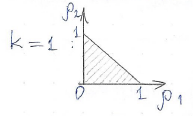
\includegraphics{pic1.png}
  \end{figure}

  \[
    x_k(t) =
    \left\{
      \begin{aligned}
        &1 - kt, &\quad t \in \left[0, \frac{1}{k}\right], \\
        &0, &\quad \text{иначе},
      \end{aligned}
    \right.
  \]
  отвечающую управлению
  \[
    u_k(t) =
    \left\{
      \begin{aligned}
        &-k, &\quad t \in \left[0, \frac{1}{k}\right], \\
        &0, &\quad \text{иначе}.
      \end{aligned}
    \right.
  \]
  Тогда $J[u_k(\cdot)] = \int\limits_0^{\frac{1}{k}}(-1 + kt)^2 dt = \dfrac{1}{3k} \To\limits_{k \to +\infty} 0$.

  Однако этот $inf$ не достигается в силу непрерывности $x$. Это плохая задача. ПМП в ней не даёт решения (см. самую первую лекцию).
\end{example}

\begin{example}
  \begin{gather*}
    \dot{x} = u, \\
    J = \int_0^1 [x^2(t) + (1 - u^2(t))^2] dt \to \inf, \\
    x(0) = x(1) = 0.
  \end{gather*}
  В этой задаче
  \begin{gather*}
    \H = \psi_0 (u_1^2 + (1 - u^2)^2) + \psi_1 u, \\
    \left\{
      \begin{aligned}
        &\dot{\psi}_0 = 0, \\
        &\dot{\psi}_1 = -2 \psi_0 x_1.
      \end{aligned}
    \right.
  \end{gather*}
  Задача автономная, значит, $\H = const$, значит,
  \[
    \psi_0[2(1 - u^2)(-2u)] + \psi_1 = 0.
  \]
  Отсюда можно найти $u^*$ и \textit{как бы} получить решение задачи.

  Покажем, что $\inf J[u(\cdot)] = 0$.

  \begin{figure}[ht!]
    \centering
    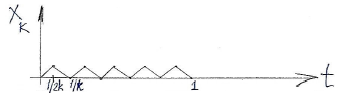
\includegraphics{pic2.png}
  \end{figure}

  Рассмотрим минимизирующую последовательность (своеобразные "пилы")
  \[
    x_k(t) = 
    \left\{
      \begin{aligned}
        t - \frac{2j}{2k}, &\quad t \in \left[\dfrac{2j}{2k}, \frac{2j + 1}{2k}\right], \\
        -t + \frac{2j + 2}{2k}, &\quad t \in \left[\dfrac{2j + 1}{2k}, \frac{2j + 2}{2k}\right],
      \end{aligned}
    \right.
  \]
  отвечающую управлению
  \[
    u_k(t) = 
    \left\{
      \begin{aligned}
        1, &\quad t \in \left[\dfrac{2j}{2k}, \frac{2j + 1}{2k}\right], \\
        -1, &\quad t \in \left[\dfrac{2j + 1}{2k}, \frac{2j + 2}{2k}\right],
      \end{aligned}
    \right.
  \]
  Тогда
  \[
    J[u_k(\cdot)] = k \int\limits_0^{\frac{1}{k}} x_k^2(t) dt = 2k \int\limits_0^{\frac{1}{2k}} t^2 dt = \dfrac{1}{3(2k)^2} \To\limits_{k \to \infty} 0.
  \]
  Но этот $\inf$ не достигается по тем же причинам, что и в примере~1. При ограничениях $|u| \leqslant 1$ "--- тот же результат. Это плохая задача. ПМП при этом даёт результат, но неправильный.

  \textit{Мораль: поскольку ПМП носит необходимый характер, \\важно всегда проверять на адекватность решение, найденное через него}.
\end{example}

\begin{example}
  \begin{gather*}
    \dot{x} = u, \quad |u| \leqslant 1, \\
    t_0 = 0, \: x(0) = 0 = x^0, \\
    t_1 x(t_1) = 1, \\
    J = x(t_1) \to \inf.
  \end{gather*}
  Выписываем ограничения по нашему общему виду ПМП (здесь более простые из первой половины семестра не применимы "--- условия на концах специфичные).
  \[
    \begin{matrix}
      &\varphi_0 = x^1_1         &\quad \varphi_2 = t_0 - 0 \\
      &\varphi_1 = t_1 x^1_1 - 1 &\quad \varphi_3 = x^0_1 - 0
    \end{matrix}
  \]
  \[
    \H = \psi_1 u \quad \thus \quad
    u^* =
    \left\{
      \begin{aligned}
        1, &\quad \psi_1 > 0, \\
        [-1, 1], &\quad \psi_1 = 0, \\
        -1, &\quad \psi_1 < 0.
      \end{aligned}
    \right.
  \]
  Отсюда
  \[
    \begin{matrix}
      \dot{\psi_1} = 0 \\
      \psi_1[0] = - \lambda_3 &\quad \H \vert_{t = t_0} = \lambda_2 \\
      \psi_1[t_1] = \lambda_0 + \lambda_1 t_1 &\quad \H \vert_{t = t_1} = -\lambda_1 x(t_1)
    \end{matrix}
  \]
  Фиксируем $\tau > 0$.
  \[
    \begin{matrix}
      u(t) = 0, \; t \in [0, \tau], &\quad x(t) = 0, \\
      u(t) = 1, \; t > \tau, &\quad x(t) = t - \tau
    \end{matrix}
  \]
  \[
    x(t_1) t_1 = 0 \thus t_1^2 - \tau t_1 - 1 = 0 \thus t_1 = \dfrac{\tau + \sqrt{\tau^2 + 4}}{2}
  \]
  \[
    \tau \to \infty \thus t_1 \to \infty, \; x(t_1) = \dfrac{1}{t_1} \to 0,
  \]
  то $\inf = 0$, но он не достигается.
\end{example}

\begin{example}
  \[
    \left\{
      \begin{aligned}
        &\dot{x}_1 = -(x_2)^2 + u^2, \\
        &\dot{x}_2 = u, \\
        &|u| \leqslant 1.
      \end{aligned}
    \right.
  \]
  \[
    t_0 = 0, \: x(0) = (-1, 0)^T = x^0
  \]
  Целевое множество $\X^1 = \left\{ x_1^2 + x_2^2 = a^2 \right\}, \; a \in (0, 1)$. Критерий:
  \[
    J = t_1 \to \infty.
  \]

  \begin{figure}[ht!]
    \centering
    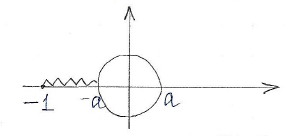
\includegraphics{pic3.png}
  \end{figure}

  Фиксируем $k \in \N, \: j = 0, \ldots, N-1$, где $N$ "--- некоторый введённый нами параметр.

  \[
    x_{2,k}(t) = 
    \left\{
      \begin{aligned}
        t - \frac{2j}{2k}, &\quad t \in \left[\dfrac{2j}{2k}, \frac{2j + 1}{2k}\right], \\
        -t + \frac{2j + 2}{2k}, &\quad t \in \left[\dfrac{2j + 1}{2k}, \frac{2j + 2}{2k}\right],
      \end{aligned}
    \right.
  \]
  отвечающую управлению
  \[
    u_k(t) = 
    \left\{
      \begin{aligned}
        1, &\quad t \in \left(\dfrac{2j}{2k}, \frac{2j + 1}{2k}\right] \bigcup \{ 0 \}, \\
        -1, &\quad t \in \left(\dfrac{2j + 1}{2k}, \frac{2j + 2}{2k}\right],
      \end{aligned}
    \right.
  \]
  
  \[ 0 \leqslant x_{2, k}(t) \leqslant \dfrac{1}{2k}, \qquad \dot{x}_1 = - x_2^2 + 1 \geqslant 1 - \dfrac{1}{(2k)^2} > 0 \]

  \[ \exists\, t_1(k) \colon x_{1,k}^2(t_1) + x_{2,k}^2(t_1) = a^2 \]

  Покажем, что $t_1(k) \To\limits_{k \to \infty} 1 - a$:
  \[
    1 - a \leqslant t_1(k) \leqslant \dfrac{1 - a}{1 - \frac{1}{(2k)^2}} + \dfrac{1}{k} \To\limits_{k \to \infty} 1 - a.
  \]
  Левая оценка следует из неравенства $\dot{x}_1 = 1 - x_2^2 \leqslant 1$ (проинтегрируем на $0, t_1(k)$ и получим результат).
  Правая оценка состоит из двух слагаемых; первое "--- время, за которое мы доезжаем до $x_1 = -a$, второе "--- время, необходимое, чтобы проехать ещё 1 "зубчик".

  Таким образом, $J_* = \inf J = 1 - a$, но этот $\inf$ не достигается.
\end{example}

\section{Достаточные условия существования решения задачи ОУ}
\begin{theorem}
  Пусть
  \[
    \dot{x}(t) = f(t, x(t), u(t)), u(t) \in \P,
  \]
  $f$ удовлетворяет основным условиям (см. лекцию про решение по Каратеодори).
  
  Задача ОУ:
  \[
    \varphi_0(e) \to \inf, \qquad \varphi_1(e) = \ldots = \varphi_k(e) = 0.
  \]

  Пусть, кроме того, выполнены следующие условия.

  \begin{itemize}
    \item[а)] Множество допустимых пар $\{ x(\cdot), u(\cdot) \}$ не пусто, т.~е.
    \[
      S' = \left\{ \left\{ t_0, t_1, x^0, u(\cdot) \right\} \in S \middle\vert \varphi(e) = 0, \; e = e(t_0, t_1, x^0, u(\cdot))  \right\} \neq \emptyset
    \] 
    (контрпример: $\dot{x} = 0, x(0) = 1, x(1) = 0$)
    \item[б)] $\P \in \mathrm{comp} \R^m$ (контрпример: пример~1)
    \item[в)] $E = \left\{ e = (t_0, x^0, t_1, x^1) \in \R^{2n + 2} \colon\; \varphi(e) = 0 \right\}$ "--- компакт, $\bar{\varphi} \in C(E)$ (контрпример: пример~3)
    \item[г)]  $\mathcal{F}(t,x) = \bigcup\limits_{u \in \P} \{f(t,x,u)\}$ "--- множество возможных скоростей (векторграмма), $\mathcal{F}(t,x) \in \mathrm{conv} \R^n$ (контрпример: примеры~2 и~4).
  \end{itemize}

  Тогда решение рассматриваемой задачи ОУ существует.
\end{theorem}
\begin{remark}
  К пункту г). 
  
  Во втором примере:
  \[
    \bar{\mathcal{F}} = \begin{bmatrix}x_1^2\\0\end{bmatrix} + \bigcup\limits_{|u| \leqslant 1} \begin{bmatrix}(1-u^2)^2\\u\end{bmatrix}
  \]
  Второе слагаемое:
  \begin{figure}[ht!]
    \centering
    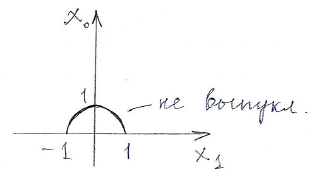
\includegraphics{pic4.png}
  \end{figure}

  В четвёртом примере:
  \[
    \bar{\mathcal{F}} = \begin{bmatrix}-x_2^2\\0\end{bmatrix} + \bigcup\limits_{|u| \leqslant 1} \begin{bmatrix}u^2\\u\end{bmatrix}
  \]
  Второе слагаемое:
  \begin{figure}[ht!]
    \centering
    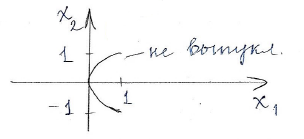
\includegraphics{pic5.png}
  \end{figure}
\end{remark}
\begin{remark}
  Иногда удобно рассматривать дифференциальное включение
  \[
    \dot{x}(t) \in \mathcal{F}(t, x(t)).
  \]
  Множество траекторий ДВ всюду плотно во множестве траекторий релаксированной задачи
  \[
    \dot{x}(t) \in \mathrm{conv} \mathcal{F}(t, x(t)),
  \]
  где $\mathrm{conv}$ "--- выпуклая оболочка.

  Как следствие, если система квазилинейна по $u$, т.~е. 
  \[
    f(t,x,u) = f^0(t,x) + G(t,x)u,
  \]
  то условие г) можно заменить на условие г') $\P \in conv \R^m$ (условие б) тогда автоматически выполнено).
\end{remark}

\begin{proof}[(теоремы)]
  Пусть $\{t_0^k, t_1^k, x^{0,k}, u_k(\cdot)\}$ "--- минимизирующая последовательность.

  В силу в),
  \[
    \min\limits_{e \in E} \varphi_0(e) \leqslant J_* = \inf J \;\thus\: J_* > -\infty.
  \]

  Выпишем определение инфинума.
  \[
    \forall \varepsilon > 0 \exists\,\{ t_0, t_1, x^0, u(\cdot) \} \colon J_* \leqslant J < J_* + \varepsilon.
  \]
  Положим $\varepsilon = \frac{1}{k}$, $e_k = (t_0^k, x^{0,k}, t_1^k, x^{1,k})$. Дано: $J(e_k) \to J_*$.

  Доказательство проведём в два этапа: сначала мы покажем, что $x_k \to x^*$, а затем "--- что эта траектория порождается некоторым допустимым управлением.

  Обозначим через $x_k(\cdot)$ траектории, отвечающие $u_k(\cdot)$. Покажем, что последовательность $\{x_k(\cdot)\}$ "--- равномерно ограничена и равностепенно непрерывна.

  \begin{enumerate}
    \item Из условия сублинейного роста: $\| f(t,x,u) \| \leqslant A \|x\| + B$ следует, что $\exists\, M_1 > 0 \colon \| x(t) \| \leqslant M_1$. Покажем, что это действительно так. Для этого продифференцируем квадрат нормы $x(t)$:
    \begin{gather*}
      \dfrac{d}{dt} \| x(t) \|^2 = 2 \left< x, f(t,x,u) \right> \leqslant \\
      \leqslant 2 \|x\| \|f\| \leqslant 2A \|x\|^2 + 2B \|x\| = (2A + 1) \|x\|^2 + \tilde{B} \\
      \thus \dfrac{d}{dt}\left(\|x(t)\|^2 \e^{-(2A+1)t}\right) \leqslant \tilde{B} \e^{-(2A + 1)t}\\
      \| x(t) \|^2 \e^{-(2A+1)t} - \norm{x(t_0)}^2 \e^{-(2A+1)t_0} \leqslant \int\limits_{t_0}^{t} \tilde{B} \e^{-(2A + 1)s} ds \\
      \norm{x_k(t)}^2 \leqslant \norm{x_k(t_0^k)} \e^{(2A + 1)(t - t_0^k)} + \e^{(2A + 1)t} \int\limits_{t_0^k}^{t} \tilde{B} \e^{-(2A + 1)s}ds.
    \end{gather*}
    Правая часть ограничена, следовательно, $\{x_k(\cdot)\}$ равномерно ограничена. Если требуется, расширяем область определения.
  
    Равностепенная непрерывность ($t' \leqslant t''$):
    \begin{gather*}
      \norm{x_k(t') - x_k(t'')} \leqslant \int\limits_{t'}^{t''} \norm{f(t, x_k(t), u_k(t))} dt \leqslant \\
      \leqslant A M_1 + B = L \abs{t'' - t'} < \varepsilon
    \end{gather*}
  
    Тогда по теореме Арцела-Асколи $x_k(\cdot) \rightrightarrows x^*(\cdot)$.
    Тогда в последнем соотношении перейдём к пределу при $k \to \infty$, получим
    \[
      \norm{x^*(t') - x^*(t'')} \leqslant L \abs{t'' - t'},
    \]
    то есть $x^* \in Lip \;\thus\: x^* \in AC$.

    \item Докажем, что $\dfrac{d x^*(t)}{dt} \in \mathcal{F}(t, x^*(t))$ для почти всех $t$.
    
    Пусть $t$ такового, что $\exists\, \frac{d}{dt}x^*(t)$. Обозначим
    \[
      \mathcal{F}_{\varepsilon, t} = \mathcal{F}_t + B_{\varepsilon}(0) \in \mathrm{conv}~\R^n.
    \]

    $f$ "--- непрерывна по $(t, x, u)$, $\exists T_0 < T_1$: $T_0 \leqslant t_0^k \leqslant t_1^k \leqslant T_1$; по теореме Кантора $f$ "--- равномерно непрерывна на $[T_0, T_1] \times B_{M_1}(0) \times \P$. Это означает, что $\forall \varepsilon > 0 \,\exists\, \delta(\varepsilon) > 0 \colon$
    \begin{gather*}
      \forall (t', x', u'), (t'', x'', u'') \in [T_0, T_1] \times B_{M_1}(0) \times \P\\
      \abs{t' - t''} + \norm{x' - x''} + \norm{u' - u''} < \delta \thus \\
      \thus \norm{f(t', x', u') - f(t'', x'', u'')} < \varepsilon
    \end{gather*}
    Возьмём $u' = u'' = u$, тогда $\forall (\tau, x) \in [T_0, T_1] \times B_{M_1}(0) \colon$
    \[
      \abs{\tau - t} + \norm{x - x^*(t)} < \delta \thus \Delta f = \norm{f(\tau, x, u) - f(t, x^*, u)} \leqslant \varepsilon
    \]
    
    По определению $\Delta f$: $\forall u \in \P \thus  f(\tau, x, u) = f(t, x^*(t), u) + \Delta f$. Отсюда
  \[
    \mathcal{F}(\tau, x) = \bigcup\limits_{u \in \P} \left\{ f(\tau,x,u) \right\} \subseteq \bigcup\limits_{u \in \P} \left\{ f(t,x^*,u) \right\} + \varepsilon B_1(0) = \mathcal{F}_{\varepsilon, t}.
  \]

  Рассмотрим неравенство 
  \[
    \norm{x_k(\tau) - x^*(t)} \leqslant \norm{x_k(\tau) - x_k(t)} + \norm{x_k(t) - x^*(t)}.
  \]

  В силу равномерной сходимости $x_k$: $\exists K \colon \abs{\tau - t} < \tilde{\delta} \leqslant \frac{\delta}{2}$ 
  \[
    \forall k \geqslant K \thus \norm{x_k(t) - x^*(t)} \leqslant \frac{\delta}{4}.
  \]

  Для первого слагаемого: $\norm{x_k(\tau) - x_k(t)} \leqslant L \abs{\tau - t} < \frac{\delta}{4}$, при этом будем выбирать $\tau$ таким, чтобы выполнялось $\abs{\tau - t} < \min(\frac{\delta}{4L}, \frac{\delta}{2})$.

  Таким образом, $\mathcal{F}(\tau, x_k(\tau)) \subseteq \mathcal{F}_{\varepsilon, t}$.

  Рассмотрим последовательность
  \[
    z_k(s) = f(s, x_k(s), u_k(s)).
  \]
  Для неё
  \[
    \dfrac{x_k(t+h) - x_k(t)}{h} = \dfrac{1}{h} \int\limits_{t}^{t+h} z_k(s) ds,
  \]
  $\abs{h} < \tilde{\delta}$, $t + h \in [T_0, T_1]$.

  $z_k(s) \in \mathcal{F}(s, x_k(s)) \subseteq \mathcal{F}_{\varepsilon, t} \thus$ (в силу г))
  \[
    \dfrac{1}{h} \int\limits_{t}^{t+h} z_k(s) ds \in \mathcal{F}_{\varepsilon, t}.
  \]

  \begin{gather*}
    \thus \left. \dfrac{x_k(t+h) - x_k(t)}{h} \in \mathcal{F}_{\varepsilon, t} \qquad \right\vert \lim\limits_{k \to \infty} \\
    \thus \left. \dfrac{x^*(t+h) - x^*(t)}{h} \in \mathcal{F}_{\varepsilon, t} \qquad \right\vert \lim\limits_{h \to \infty} \\
    \thus \left. \dfrac{d x^*(t)}{dt} \in \mathcal{F}_{\varepsilon, t} \; \forall \varepsilon > 0 \qquad \right\vert \lim\limits_{\varepsilon \to 0 + 0} \\
    \thus \dfrac{d x^*(t)}{dt} \in \mathcal{F}(t, x^*(t)).
  \end{gather*}

  Как найти $u^*(\cdot)$?
  \[
    \dfrac{dx^*(t)}{dt} = \{ \text{п.~в. } t \} = f(t, x^*(t), u^*(t))\\ 
  \]
  Рассмотрим
  \[  
    \P^*(t) = \left\{ u \in \P \colon f(t, x^*(t), u) = \dfrac{dx^*(t)}{dt} \right\}.
  \]
  $\P^*$ определена во всех точках $t$, где $\exists \dfrac{dx^*}{dt}$, $\P^* \neq \emptyset$

  Верно ли, что $\P^*$ "--- измеримо по $t$?

  Для использования теоремы Лузина надо показать, что 
  \begin{gather*}
    \forall \tilde{\varepsilon} < 0 \colon \{ \exists\, \tilde{T}_0, \tilde{T}_1 \colon T_0 \leqslant \tilde{T}_0 < \tilde{T}_1 \leqslant T \} \\
    \exists\, Z \subseteq [T_0, T_1] \colon \mu(Z) < \tilde{\varepsilon} \colon
  \end{gather*}
  $\P^* \vert_{[T_0, T_1] \setminus Z}$ "--- п/н сверху \textit{(ослабили непрерывность)}.

  $\dfrac{dx^*}{dt}$ "--- измерима, возьмём $Z$ такое, что $\dfrac{dx^*}{dt}$ непрерывна на $[T_0, T_1] \setminus Z$.

  $t_k \in [T_0, T_1] \setminus Z, \qquad t_k \To\limits_{k \to \infty} \bar{t}$

  Тогда
  \begin{gather*}
    u_k \in \P^*(t_k) \to \bar{u} \in \P \\
    \dfrac{dx^*(t_k)}{dt} = f(t_k, x^*(t_k), u_k) \To\limits_{k \to \infty} f(\bar{t}, x^*(\bar{t}, \bar{u})), \\
    \dfrac{dx^*(t_k)}{dt} \to \dfrac{dx^*(\bar{t})}{dt}.
  \end{gather*}

  Таким образом, $\bar{u} \in \P^*(\bar{t})$, следовательно, $\P^*$ "--- измеримо $\thus$ существует измеримый селектор $u^*(t) \in \P^*(t)$.
  \end{enumerate}
Теорема доказана.
\end{proof}
\begin{remark}
  Компактность $E$ можно заменить на компактность $E \cap \{ e \colon \varphi_k(e) \leqslant \mu \}$, где $\mu > J_*$.
\end{remark}

\end{document}